\documentclass[border=4pt]{standalone}
% Shared by the independently buildable vector figures.
\usepackage[T1]{fontenc}
\usepackage{amsmath,amssymb,newpxtext,newpxmath}
\usepackage[semibold]{sourcesans}
\usepackage{pgfplots}
\pgfplotsset{compat=1.18}
\usetikzlibrary{arrows.meta,calc,positioning}
\usepgfplotslibrary{groupplots}
\definecolor{ink}{HTML}{19303A}
\definecolor{sea}{HTML}{00675E}
\definecolor{clay}{HTML}{A24725}
\definecolor{muted}{HTML}{4C636C}
\definecolor{rulegray}{HTML}{CAD4D4}
\definecolor{wash}{HTML}{EAF4F0}
\definecolor{warm}{HTML}{F7EEE5}
\color{ink}
\tikzset{every picture/.style={font=\sffamily\small},
  arrow/.style={-{Stealth[length=2mm]},line width=.8pt,draw=muted}}
\pgfplotsset{companion/.style={axis lines=left,axis line style={draw=muted},
  tick style={draw=muted},ticklabel style={font=\sffamily\footnotesize,text=muted},
  label style={font=\sffamily\small},grid=major,grid style={draw=rulegray!64,line width=.25pt},
  tick align=outside,enlarge x limits=false,scaled ticks=false,
  every axis plot/.append style={line join=round},
  legend style={draw=none,fill=none,font=\sffamily\footnotesize},
  title style={font=\sffamily\bfseries\small,anchor=south west,at={(0,1.03)}}}}

\begin{document}
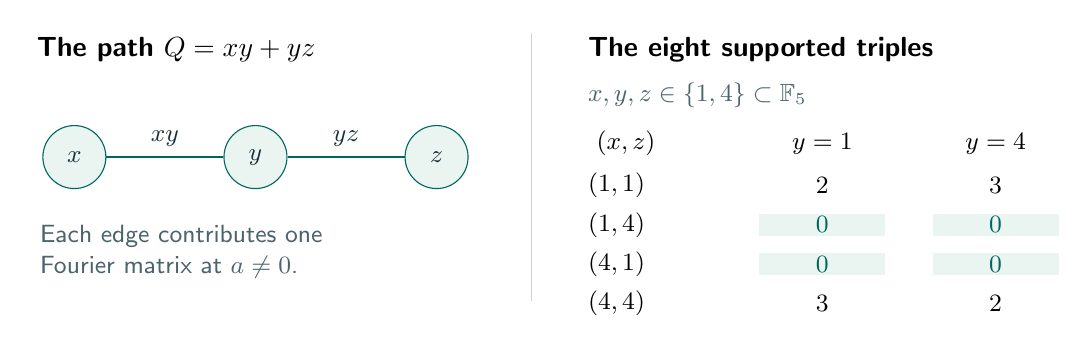
\begin{tikzpicture}[x=1cm,y=1cm]
\node[anchor=west,font=\sffamily\bfseries] at (0,3.15) {The path $Q=xy+yz$};
\foreach \a/\b in {0.6/x,2.9/y,5.2/z}{
  \node[circle,minimum size=.8cm,fill=wash,draw=sea,text=ink] (\b) at (\a,1.78){$\b$};}
\draw[thick,sea] (x) -- node[above,text=ink] {$xy$} (y);
\draw[thick,sea] (y) -- node[above,text=ink] {$yz$} (z);
\node[anchor=west,align=left,text=muted] at (.04,.58)
  {Each edge contributes one\\Fourier matrix at $a\ne0$.};
\draw[rulegray] (6.4,-.05)--(6.4,3.35);
\node[anchor=west,font=\sffamily\bfseries] at (7,3.15) {The eight supported triples};
\node[anchor=west,text=muted] at (7,2.56) {$x,y,z\in\{1,4\}\subset\mathbb F_5$};
\node[anchor=west] at (7,1.95) {$\ (x,z)$};
\node at (10.1,1.95) {$y=1$};
\node at (12.3,1.95) {$y=4$};
\foreach \pair/\ya/\a/\b in {{(1,1)}/1.42/2/3,{(1,4)}/.92/0/0,{(4,1)}/.42/0/0,{(4,4)}/-.08/3/2}{
  \node[anchor=west] at (7,\ya) {$\pair$};
  \foreach \x/\v in {10.1/\a,12.3/\b}{
    \ifnum\v=0 \node[fill=wash,text=sea,minimum width=1.6cm,inner sep=1pt] at (\x,\ya) {$0$};
    \else \node at (\x,\ya) {$\v$};\fi}}
\end{tikzpicture}
\end{document}
